\documentclass[reprint,english,notitlepage]{revtex4-1}
% if you want a single-column, remove reprint

% allows special characters (including æøå)
\usepackage[utf8]{inputenc}
\usepackage [norsk]{babel} %if you write norwegian
%\usepackage[english]{babel}  %if you write english


\usepackage{physics,amssymb}  % mathematical symbols (physics imports amsmath)
\usepackage{graphicx}         % include graphics such as plots
\usepackage{xcolor}           % set colors
\usepackage{hyperref}         % automagic cross-referencing (this is GODLIKE)
\usepackage{tikz}             % draw figures manually
\usepackage{listings}         % display code
\usepackage{subfigure}        % imports a lot of cool and useful figure commands
\usepackage{float}			  % force placement of tables and figures
\usepackage{amsmath}
\usepackage{minted}

\hypersetup{ % this is just my personal choice, feel free to change things
	colorlinks,
	linkcolor={red!50!black},
	citecolor={blue!50!black},
	urlcolor={blue!80!black}}

%% Defines the style of the programming listing
%% This is actually my personal template, go ahead and change stuff if you want
\lstset{ %
	inputpath=,
	backgroundcolor=\color{white!88!black},
	basicstyle={\ttfamily\scriptsize},
	commentstyle=\color{magenta},
	language=Python,
	morekeywords={True,False},
	tabsize=4,
	stringstyle=\color{green!55!black},
	frame=single,
	keywordstyle=\color{blue},
	showstringspaces=false,
	columns=fullflexible,
	keepspaces=true}

\begin{document}
	
\title{FYS4150 - Prosjekt 2}
\date{\today}               
\author{Karl Henrik Fredly}
\affiliation{Universitetet i Oslo} 

\newpage
	
\begin{abstract} %------------------Abstract-----------------------
	I dette prosjektet løser vi tre ulike diffligninger ved å diskretisere de og sette de opp som egenverdiproblemer. Den første ligningen finner formen til en bøyende bjelke. Den andre finner den radielle komponenten til bølgefunksjonen til et elektron i et harmonisk oscillator potensial. Den tredje finner avstanden mellom to interagerende elektroner i et harmonisk oscillator potensial.
	
	Vi bruker Jacobis egenverdialgoritme til å løse ligningene. Vi finner at Jacobis egenverdialgoritme gir så godt som samme resultater som C++ funksjoner fra biblioteket Armadillo, og som den analytiske løsningen for den bøyende bjelken. Men den er mye treigere, og bruker 38.2s på en utregning Armadillo fullførte fortere enn maskinen klarte å måle.
	
	For de kvantemekaniske systemene såg vi at vi måtte finne balansen mellom antall målepunkter og endepunktet i beregningene våre. Den numeriske metoden tilnærmet fortsatt den analytiske løsningen godt.
	
	Til slutt observerte vi et samspill mellom harmonisk oscillator potensialet og den frastøtende Coulombkraften, der vi såg at rekkevidden til Coulombkraften førte til større forskjell i avstanden mellom elektronene for svake potensialer enn for sterke.
	
	- Github repository link med all kode og resultater med ekstra forklaringer: \href{https://github.com/KarlHenrik/ComputationalPhysicsMaster/tree/master/FYS4150/Project2}{https://github.com/KarlHenrik/ComputationalPhysicsMaster/tree/master/FYS4150/Project2}
\end{abstract}
\maketitle

\section{Introduksjon} %------------------Introduksjon-----------------------
	Løsningen av diffligninger som egenverdiproblemer er et kraftig verktøy som lar oss gjøre mange forenklinger ved å bruke nyttige metoder og resultater fra blant annet lineær algebra. Dette prosjektet illustrerer hvordan svært ulike fysiske systemer lar seg løse på helt samme vis, noe som alltid er en stor fordel siden det sparer oss mye arbeid og siden det lettere lar oss se sammenhenger mellom ulike problemer.
	
	Til dette prosjektet har jeg benyttet kode som implementerer Jacobis egenverdialgoritme \cite{eigvalEmne}, med justeringer. Oppsett av matrisene og lagring av resultater implementerte jeg selv \cite{myRepo}. Jeg har også skrevet kode for å bearbeide og presentere resultatene fra denne koden \cite{myRepo}.

\section{Metoder} %------------------Metoder-----------------------
	Vi skal numerisk løse ulike diffligninger som egenverdiproblemer. Den sentrale idéen er å diskretisere diffligningen slik at vi får en matrise-egenverdi ligning. Så diagonaliserer vi matrisen vår til en similær diagonal matrise for å få egenverdiene og egenvektorene. Vi ser først hvordan vi får matrise-egenverdi ligningene før vi ser på hvordan vi løser de med Jacobi-egenverdialgoritme.
	
\subsection{Bøyende bjelke}
	
	En bjelke som blir påført en kraft $F$ ved endene $(0, L)$ innover bjelken får en avbøyning $u(x)$ (som vi skal finne) ved posisjon $x$ som følger ligningen
	
	\begin{equation*}
	\gamma \frac{d^2 u(x)}{dx^2} = -F u(x)
	\end{equation*}
	
	Hvor $\gamma$ er en materialkonstant. Vi krever at avbøyingen ved endepunktene er $u(0) = u(L) = 0$ (Dirichlet grensebetingelser). Definerer vi $\rho = \frac{x}{L}$ og $\lambda = FL^2/\gamma$ får vi ligningen av $\rho$ for $\rho \in [0,1]$
	
	\begin{equation*}
	\frac{d^2 u(\rho)}{d\rho^2} = -\lambda u(\rho),
	\end{equation*}
	
	Vi kan diskretisere denne ligningen ved å tilnærme den andrederiverte
	
	\begin{equation*}
	\frac{u(\rho+h) -2u(\rho) +u(\rho-h)}{h^2} + O(h^2) = -\lambda u(\rho),
	\end{equation*}
	
	hvor $h$ er steglengden i diskreteringen vår. Vi tar ikke med feilleddet videre i utregningen. Hvis vi har N punkter for $\rho$ får vi $h = 1/N$. Vi skriver da 
	\begin{equation*}
	\begin{aligned}
	\rho_i = ih \hspace{1cm} i=1,2,\dots , N \\
	u_i = u(\rho_i) \hspace{1cm} i=1,2,\dots , N
	\end{aligned}
	\end{equation*}
	Og vi kan skrive ligningen vår som
	\begin{equation*}
	-\frac{u_{i+1} -2u_i +u_{i-1} }{h^2}  = \lambda u_i
	\end{equation*}
	Definerer
	\begin{equation*}
	\begin{aligned}
	d&=\frac{2}{h^2} \\
	e &= -\frac{1}{h^2}
	\end{aligned}
	\end{equation*}
	Siden $u_0 = u_N = 0$ kan vi skrive disse $N - 1$ ikke-trivielle ligningene som en matriseligning
	\begin{equation*}
	\begin{bmatrix} d& a & 0   & 0    & \dots  &0     & 0 \\
	a & d & a & 0    & \dots  &0     &0 \\
	0   & a & d & a  &0       &\dots & 0\\
	\dots  & \dots & \dots & \dots  &\dots      &\dots & \dots\\
	0   & \dots & \dots & \dots  &a  &d & a\\
	0   & \dots & \dots & \dots  &\dots       &a & d\end{bmatrix} 
	\begin{bmatrix} u_1 \\ u_2 \\ u_3 \\ \dots \\ u_{N-2} \\ u_{N-1}\end{bmatrix}
	= \lambda \begin{bmatrix} u_1 \\ u_2 \\ u_3 \\ \dots \\ u_{N-2} \\ u_{N-1}\end{bmatrix}
	\end{equation*}
	
	Vi skal løse dette egenverdiproblemet numerisk for å finne de mulige verdiene $\lambda$ (som sier noe om egenskapene til bjelken) og verdiene $u_i$ som tilfredstiller ligningen (som gir de mulige formene til den avbøyde bjelken).
	Dette egenverdiproblemet har analytiske løsninger vi kan bruke til å vurdere den numeriske løsningen. Egenverdiene er gitt ved:
	\begin{equation*}
	\lambda_j = d+2a\cos{(\frac{j\pi}{N})}, \hspace{0.2cm} j=1,2,\dots N-1.
	\end{equation*}
	og egenvektorene:
	\begin{equation*}
	\begin{aligned}
	\mathbf{u}_j = [ \sin(\frac{j\pi}{N}), \sin(\frac{2j\pi}{N}), ..., \sin(\frac{(N-1)j\pi}{N}) ]^T,\\ \hspace{0.2cm} j=1,\dots N-1
	\end{aligned}
	\end{equation*}
	
\subsection{Elektron i harmonisk oscillator potensial}
	
	Et elektron i et harmonisk oscillator potensial $V(r) = \frac{1}{2}kr^2 = \frac{1}{2}m\omega^2r^2$ beskrives av en bølgefunksjon som følger Schrödingerligningn. Vi antar sfærisk symmetri om senteret til potensialet, og ser kun på den radielle delen av Schrödingerligningn. 
	\begin{equation*}
	-\frac{\hbar^2}{2 m} \left ( \frac{1}{r^2} \frac{d}{dr} r^2
	\frac{d}{dr} - \frac{l (l + 1)}{r^2} \right )R(r) 
	+ V(r) R(r) = E R(r).
	\end{equation*}
	hvor $R(r)$ er den radielle delen av bølgefunksjonen(som vi skal finne). $|R(r)|^2$ beskriver sannsynligheten for å observere elektronet i en avstand $r$ fra sentrum av potensialet.
	
	$E$ er energien til den harmoniske oscillatoren. $\omega$ er oscillatorfrekvensen og de mulige energiene er
	\begin{equation*}
	E_{nl}=  \hbar \omega \left(2n+l+\frac{3}{2}\right),
	\end{equation*}
	med $n=0,1,2,\dots$ og $l=0,1,2,\dots$. Hvor $n$ er energikvantetallet og $l$ er orbitalmomentet kvantetallet. Vi ser her kun på tilfellet $l = 0$.
	
	Vi substituerer $R(r) = (1/r) u(r)$ og $\rho = (1/\alpha) r$. Har da at $u(0) = u(\infty) = 0$ (krever alltid null sannsynlighet for å finne elektron uendelig langt unna).
	
	Setter $\alpha = \left(\frac{\hbar^2}{mk}\right)^{1/4}$ og $\lambda = \frac{2m\alpha^2}{\hbar^2}E$. Da kan vi skrive om ligningen vår til: (se \cite{oppgavetekst} for mer motivert utregning)
	
	\begin{equation*}
	-\frac{d^2}{d\rho^2} u(\rho) + \rho^2u(\rho)  = \lambda u(\rho) .
	\end{equation*}
	
	Vi kan diskretisere denne ligningen på samme vis som for den bøyende bjelken. Vi definerer på nytt en steglengde $h = \rho_N / N$ hvor $N$ er antall punkter og $\rho_N$ er den største verdien for $\rho$ i diskretiseringen vår. Vi kan ikke sette $\rho_N = \infty$ i den numeriske løsningen, men vi vil finne at vi får gode tilnærminger for selv relativt små $\rho_N$. Videre:
	\begin{equation*}
	\begin{aligned}
	\rho_i = ih \hspace{1cm} i=1,2,\dots , N \\
	u_i = u(\rho_i) \hspace{1cm} i=1,2,\dots , N \\
	V_i = \rho_i^2 \hspace{1cm} i=1,2,\dots , N
	\end{aligned}
	\end{equation*}
	Da blir den diskretiserte ligningen
	\begin{equation*}
	-\frac{u_{i+1} -2u_i +u_{i-1} }{h^2}+V_iu_i  = \lambda u_i
	\end{equation*}
	Definerer
	\begin{equation*}
	\begin{aligned}
	d_i&=\frac{2}{h^2}+V_i \\
	e &= -\frac{1}{h^2}
	\end{aligned}
	\end{equation*}
	Siden $u(0) = u(\rho_N) = 0$ kan skrive disse ikke-trivielle ligningene som en matriseligning
	\begin{equation*}
	\begin{bmatrix}d_1 & e & 0   & 0    & \dots  &0     & 0 \\
	e & d_2 & e & 0    & \dots  &0     &0 \\
	0   & e & d_3 & e  &0       &\dots & 0\\
	\dots  & \dots & \dots & \dots  &\dots      &\dots & \dots\\
	0   & \dots & \dots & \dots  &\dots  e     &d_{N-2} & e\\
	0   & \dots & \dots & \dots  &\dots       &e & d_{N-1}
	\end{bmatrix}  \begin{bmatrix} u_{1} \\
	u_{2} \\
	\dots\\ \dots\\ \dots\\
	u_{N-1}
	\end{bmatrix}=\lambda \begin{bmatrix} u_{1} \\
	u_{2} \\
	\dots\\ \dots\\ \dots\\
	u_{N-1}
	\end{bmatrix}
	\end{equation*}
	Vi skal finne egenverdiene og egenvektorene til denne matrisen numerisk ved å diagonalisere den, slik som for den bøyende bjelken. Egenverdiene $\lambda$ gir oss energien $E$ hvis vi vet $k$. Egenvektorene $u$ (ganget med r) gir oss den tilhørende bølgefunksjonen som lar oss si noe om posisjonen til elektronet.
	
	For vår skalering av problemet er de analytiske egenverdiene $\lambda=3,7,11,15,\dots$. Vi skal bruke disse til å vurdere resultatet til den numeriske løsningen.
	
\subsection{To elektron i harmonisk oscillator potensial}
	
	To elektron i et harmonisk oscillator potensial vil frastøte hverandre pga. Coulomb kraften. Dette gjør det vanskeligere å regne ut bølgefunksjonene til elektronene, men vi skal se at avstanden mellom elektronene kan finnes ved en ligning lik de vi har sett på hittil.
	Vi begynner med Schrödingerligningn for kun ett elektron
	\begin{equation*}
	-\frac{\hbar^2}{2 m} \frac{d^2}{dr^2} u(r) 
	+ \frac{1}{2}k r^2u(r)  = E^{(1)} u(r),
	\end{equation*}
	hvor $E^{(1)}$ er energien til dette ene elektronet. For to elektroner uten noen frastøtende kraft får vi
	\begin{equation*}
	\left(  -\frac{\hbar^2}{2 m} \frac{d^2}{dr_1^2} -\frac{\hbar^2}{2 m} \frac{d^2}{dr_2^2}+ \frac{1}{2}k r_1^2+ \frac{1}{2}k r_2^2\right)u(r_1,r_2)  = E^{(2)} u(r_1,r_2) .
	\end{equation*}
	hvor $E^{(2)}$ er summen av energiene til elektronene. Merk at elektronene deler følgefunksjon $u(r_1, r_2)$ siden vi ikke kan skille mellom hvilket elekton vi observerer. Vi introduserer den relative koordinaten $\mathbf{r} = \mathbf{r}_1-\mathbf{r}_2$ og massesenterkoordinaten $\mathbf{R} = 1/2(\mathbf{r}_1+\mathbf{r}_2)$. Med disse skriver vi om ligningen
	\begin{equation*}
	\left(  -\frac{\hbar^2}{m} \frac{d^2}{dr^2} -\frac{\hbar^2}{4 m} \frac{d^2}{dR^2}+ \frac{1}{4} k r^2+  kR^2\right)u(r,R)  = E^{(2)} u(r,R).
	\end{equation*}
	Vi kan separere bølgefunksjonen $u(r,R) = \psi(r)\phi(R)$. Vi kan også separere energien $E^{(2)}=E_r+E_R$. Videre ser vi kun på bølgefunksjonen og energien tilhørende den relative posisjonen, og vi legger til et potensial fra Coulomb-kraften.
	\begin{equation*}
	V(r_1,r_2) = \frac{\beta e^2}{|\mathbf{r}_1-\mathbf{r}_2|}=\frac{\beta e^2}{r},
	\end{equation*}
	hvor $\beta e^2=1.44$ eVnm. Vi får da totalt
	\begin{equation*}
	\left(  -\frac{\hbar^2}{m} \frac{d^2}{dr^2}+ \frac{1}{4}k r^2+\frac{\beta e^2}{r}\right)\psi(r)  = E_r \psi(r).
	\end{equation*}
	Definerer 
	\begin{equation*}
	\begin{aligned}
	\omega_r^2=\frac{1}{4}\frac{mk}{\hbar^2} \alpha^4 \\
	\alpha = \frac{\hbar^2}{m\beta e^2} \\
	\lambda = \frac{m\alpha^2}{\hbar^2}E
	\end{aligned}
	\end{equation*}
	og skriver om Schrödingerligningn vår til
	\begin{equation*}
	-\frac{d^2}{d\rho^2} \psi(\rho) + \omega_r^2\rho^2\psi(\rho) +\frac{1}{\rho} = \lambda \psi(\rho).
	\end{equation*}
	
	Vi kan diskretisere denne ligningen på samme vis som før. Vi definerer en steglengde $h = \rho_N / N$ hvor $N$ er antall punkter og $\rho_N$ er den største verdien for $\rho$ i diskretiseringen vår. Vi kan ikke sette $\rho_N = \infty$ i den numeriske løsningen, men vi vil finne at vi får gode tilnærminger for selv relativt små $\rho_N$. Videre:
	\begin{equation*}
	\begin{aligned}
	\rho_i = ih \hspace{1cm} i=1,2,\dots , N \\
	u_i = \psi(\rho_i) \hspace{1cm} i=1,2,\dots , N \\
	V_i = \omega_r^2 \rho_i^2 + \frac{1}{\rho} \hspace{1cm} i=1,2,\dots , N
	\end{aligned}
	\end{equation*}
	Da blir den diskretiserte ligningen
	\begin{equation*}
	-\frac{u_{i+1} -2u_i +u_{i-1} }{h^2}+V_iu_i  = \lambda u_i
	\end{equation*}
	Definerer
	\begin{equation*}
	\begin{aligned}
	d_i&=\frac{2}{h^2}+V_i \\
	e &= -\frac{1}{h^2}
	\end{aligned}
	\end{equation*}
	Siden $u(0) = u(\rho_N) = 0$ kan skrive disse ikke-trivielle ligningene som en matriseligning
	\begin{equation*}
	\begin{bmatrix}d_1 & e & 0   & 0    & \dots  &0     & 0 \\
	e & d_2 & e & 0    & \dots  &0     &0 \\
	0   & e & d_3 & e  &0       &\dots & 0\\
	\dots  & \dots & \dots & \dots  &\dots      &\dots & \dots\\
	0   & \dots & \dots & \dots  &\dots  e     &d_{N-2} & e\\
	0   & \dots & \dots & \dots  &\dots       &e & d_{N-1}
	\end{bmatrix}  \begin{bmatrix} u_{1} \\
	u_{2} \\
	\dots\\ \dots\\ \dots\\
	u_{N-1}
	\end{bmatrix}=\lambda \begin{bmatrix} u_{1} \\
	u_{2} \\
	\dots\\ \dots\\ \dots\\
	u_{N-1}
	\end{bmatrix}
	\end{equation*}
	Vi skal finne egenverdiene og egenvektorene til denne matrisen numerisk ved å diagonalisere den, slik som for den bøyende bjelken. Egenverdiene $\lambda$ gir oss energien $E$. Egenvektorene $u$ gir oss den tilhørende bølgefunksjonen som lar oss si noe om avstanden mellom elektronene.
	
	Vi skal se hva som skjer for $\omega_r = 0.01, 0.5, 1, 5$, altså hva som skjer for et svakt eller sterkt harmonisk oscillator potensial for grunntilstanden (tilstanden med lavest energi/egenverdi).
	
\subsection{Jacobi-egenverdialgoritme}
	Denne diskusjonen rundt Jacobis egenverdialgoritme baserer seg på FYS4150 kursmateriell \cite{eigvalEmne}. Her kommer jeg bare til å gå gjennom de sentrale ideene, og ikke alle detaljene.
	
	Vi har en symmetrisk matrise $A$ som vi vil finne egenverdiene og egenvektorene til. Hvis vi finner en diagonal matrise $D$ som er similær med $A$ vil de per def. ha samme egenverdier, og siden $D$ er diagonal vil disse bare være diagonalelementene til $D$.
	
	Målet er å finne en unitær similær transformasjon $S$ slik at $D = S^T A S$ hvor $S^T S = S^{-1}S = I$.
	
	Anta $x$ er en egenvektor til $A$. Da har vi $Ax = \lambda x$, og dermed $SDS^T x = \lambda x$ og til slutt $D(S^Tx) = \lambda (S^Tx)$. $S^T x$ er en egenvektor til $D$ med egenverdi $\lambda$, men egenvektorene til en diagonal matrise er standardbasisvektorene, så vi kan finne egenvektorene $x$ til A ved å begynne med standardbasisvektorene og multiplisere med $S$ fra venstre.
	
	Unitære transformasjoner $w_i = Uv_i$ bevarer prikk produktet og ortogonaliteten $v_j^T v_i = \delta_{ij}$ siden $w_j^T w_i = (Uv_j)^T (Uv_i) = v_j^T U^TUv_i = v_j^T v_i$.
	
	Jacobis egenverdialgoritme går ut på å bruke flere transformasjoner $S$ på formen
	\begin{equation*}
	\mathbf{S}=
	\left( 
	\begin{array}{cccccccc}
		1  &    0  & \dots &   0        &    0  & \dots & 0 &   0       \\
		0  &    1  & \dots &   0        &    0  & \dots & 0 &   0       \\
		\dots & \dots & \dots & \dots      & \dots & \dots & 0 & \dots     \\ 
		0  &    0  & \dots & \cos\theta  &    0  & \dots & 0 & \sin\theta \\
		0  &    0  & \dots &   0        &    1  & \dots & 0 &   0       \\
		\dots & \dots & \dots & \dots      & \dots & \dots & 1 & \dots     \\
		0  &    0  & \dots &  -\sin\theta        &    0  & \dots & 0 &   \cos\theta   
	\end{array}
	\right)
	\end{equation*}
	disse kan ses på som en plan-rotasjon med vinkel $\theta$ i det euklidiske n-dimensjonelle rommet. Man velger plasseringen av cos og sin leddene slik at $S^T A S$ er nærmere diagonal enn $A$. Det dette betyr i praksis er å finne det største elementet i $A$ og velge $S$ slik at dette settes til 0 på begge sider av diagonalen (hugs at $A$ er symmetrisk). De andre elementene i $A$ som deler rad og kolonne med det største elementet i $A$ (på begge sider av diagonalen) vil også endres, men summen av størrelsen til elementene som ikke er på diagonalen til $A$ vil bli mindre \cite{eigvalEmne}.
	
	Først finner vi plasseringen til de største elementene i $A$ ($a_{kl}$ og $a_{lk}$) (på hver sin side av diagonalen). Plasserer vi cos og sin leddene i $S$ i samme rader og kolonner (l og k) og setter leddene med indeks kl og lk i $S^T A S$ lik 0 får vi denne ligningen:
	\begin{equation*}
	\tan(\theta) = -\tau \pm \sqrt{1 - \tau^2}
	\end{equation*}
	hvor vi brukte at
	\begin{equation*}
	\cot 2\theta= \tau = \frac{a_{ll}-a_{kk}}{2a_{kl}}
	\end{equation*}
	Dette lar oss finne $\theta$ og dermed $S$ som lar oss komme nærmere en similær diagonal matrise $D$ (i praksis finner vi bare $sin\theta$ og $cos\theta$)). Gjør vi dette nok ganger ender vi opp med en matrise som har små nok elementer av diagonalen at den er tilnærmet diagonal.
	

\section{Resultater} %------------------Resultater-----------------------
	
\subsection{Jacobi-egenverdialgoritme ytelse}
	Vi løser ligningene for den bøyende bjelken analytisk, med funksjoner fra C++ biblioteket Armadillo og med Jacobi-egenverdialgoritmen, og sammenligner tiden de tar.
	
	\begin{table}[H]
		\begin{center}
			\caption{Tid (s) det tok for hver metode å løse å løse bøyende bjelke ligningen for ulike antall punkter.}
			\label{tab:time}
			\begin{tabular}{|c|c|c|c|} \hline
				\textbf{$n$} & \textbf{Analytisk} & \textbf{Armadillo} & \textbf{Jacobi} \\ \hline
				100 & 0.01 & 0.00 & 0.17 \\
				200 & 0.01 & 0.00 & 2.41 \\
				300 & 0.04 & 0.00 & 12.5 \\
				400 & 0.09 & 0.00 & 38.3 \\ \hline
			\end{tabular}
		\end{center}
	\end{table}

	Vi ser også på hvor mange iterasjoner av Jacobi-egenverdialgoritme som var nødvendig for at alle ikke-diagonale elementene var så godt som null ($< 10^{-10}$).
	\begin{table}[H]
		\begin{center}
			\caption{Nødvendige iterasjoner av Jacobi-egenverdialgoritme for ulike antall punkter.}
			\label{tab:iters}
			\begin{tabular}{|c|c|} \hline
				\textbf{$n$} & \textbf{Iterasjoner} \\ \hline
				100 & 18773 \\
				200 & 74944 \\
				300 & 170278 \\
				400 & 301772 \\ \hline
			\end{tabular}
		\end{center}
	\end{table}

\subsection{Bøyende bjelke løsning}
	Ved å løse ligningen for den bøyende bjelken for 100 punkter får vi disse minste egenverdiene:
	\begin{table}[H]
		\begin{center}
			\caption{De fire minste egenverdiene for den bøyende bjelken for de ulike metodene. De er helt like, og med flere siffer enn det som er fint å se på ser vi at de alle er like for de første 10 sifrene.}
			\label{tab:bbeig}
			\begin{tabular}{|c|c|c|} \hline
				\textbf{Analytisk} & \textbf{Armadillo} & \textbf{Jacobi} \\ \hline
				9.868 & 9.868 & 9.868 \\
				39.46 & 39.46 & 39.46 \\
				88.76 & 88.76 & 88.76 \\
				157.7 & 157.7 & 157.7\\ \hline
			\end{tabular}
		\end{center}
	\end{table}
	Vi fikk også egenvektorene tilhørende alle egenverdiene. Plotter her egenvektoren for den minste egenverdien funnet analytisk og med Jacobi.
	\begin{figure}[H]
		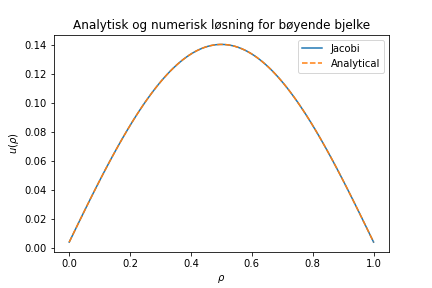
\includegraphics[width=90mm]{../Figures/bjelke1.png}
		\caption{Egenvektor for ligningen til den bøyende bjelken tilhørende den laveste egenverdien. Sammenligner her den analytiske løsningen med løsningen funnet med Jacobis egenverdialgoritme.}
		\label{fig:bb}
	\end{figure}
	De andre egenvektorene svinger flere ganger om sentrum. Neste egenvektor svinger én gang om midten, neste deretter to ganger osv.
	
\subsection{Ett elektron løsning}
	For å analysere effekten av å endre antall integrasjonpunkter $N$ og maksverdi $\rho$ regnet vi ut den første egenverdien for ulike kombinasjoner av disse.
	\begin{table}[H]
		\begin{center}
			\caption{Absolutt feil i den første egenverdien for ulike kombinasjoner av $N$ og $rho_N$ når vi løser ligingen for ett elektron}
			\label{tab:rhoN}
			\begin{tabular}{|c|c|c|c|c|} \hline
				\textbf{n/$\rho_N$} & \textbf{3} & \textbf{6} & \textbf{9} & \textbf{12} \\ \hline
				50 & 0.01108 & 0.00433 & 0.00976 & 0.01741\\
				100 & 0.01188 & 0.00110 & 0.00248 & 0.00441\\
				150 & 0.01203 & 0.00049 & 0.00111 & 0.00197\\
				200 & 0.01209 & 0.00027 & 0.00062 & 0.00111\\
				250 & 0.01211 & 0.00017 & 0.00040 & 0.00071\\ \hline
			\end{tabular}
		\end{center}
	\end{table}

	Ved et kjapt manuelt søk fant vi at $N = 300$ og $\rho_N = 6$ gav fire riktige sifre for den første egenverdien (som skal være lik 3), men fire riktige sifre for et betydelig antall egenverdier fikk vi ikke for hensiktsmessige $N$.
	
	Vi plotter egenvektorene tilhørende de tre minste egenverdiene kvadrert.
	\begin{figure}[H]
		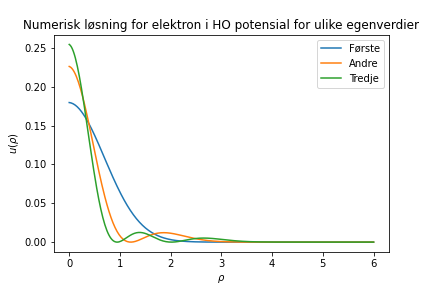
\includegraphics[width=90mm]{../Figures/ettElektron.png}
		\caption{Løsninger av ligningen for elektron i HO potensial, her: Egenvektorene tilhørende de tre minste egenverdiene kvadrert. Funnet med Jacobis egenverdialgoritme. Merk at dette er løsningen av difflikningen, ganget med $\rho$, for å få den radielle bølgefunksjonen tilbake.}
		\label{fig:ettelektron}
	\end{figure}

\subsection{To elektron løsning}
	Vi løste ligningen for to elektroner for $\omega_r = 0.01$, $\omega_r = 0.5$, $\omega_r =1$,
	og $\omega_r = 5$.
	
	Plotter egenvektorene til den laveste egenverdien (grunntilstanden) kvadrert for ulik $\omega_r$. 
	\begin{figure}[H]
		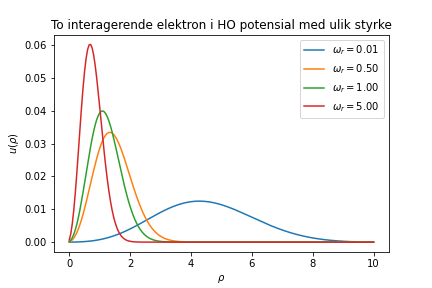
\includegraphics[width=90mm]{../Figures/toElektron.png}
		\caption{Løsninger av ligningen for to elektron i HO potensial, her: løsningene for $\omega_r = 0.01$, $\omega_r = 0.5$, $\omega_r =1$, og $\omega_r = 5$. Funnet med Jacobis egenverdialgoritme.}
		\label{fig:toelektron}
	\end{figure}

	Plotter egenvektorene til den laveste egenverdien (grunntilstanden) kvadrert for ulik $\omega_r$ uten noen frastøtende Coulomb kraft mellom elektronene.
	\begin{figure}[H]
		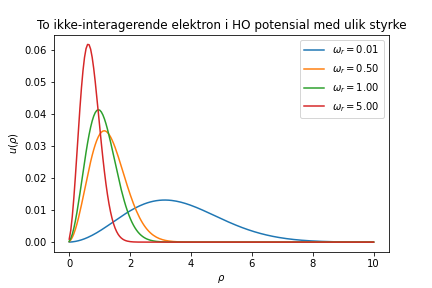
\includegraphics[width=90mm]{../Figures/toElektronNoC.png}
		\caption{Løsninger av ligningen for to elektron i HO potensial, uten Coulomb ledd, her: løsningene for $\omega_r = 0.01$, $\omega_r = 0.5$, $\omega_r =1$, og $\omega_r = 5$. Funnet med Jacobis egenverdialgoritme.}
		\label{fig:toelektronnoC}
	\end{figure}
	
\section{Diskusjon} %------------------Diskusjon-----------------------
	Tiden det tok å finne de analytiske løsningene til den bøyende bjelken er ikke av interesse, siden det kun var evalueringen av trigonometriske funksjoner for å finne hvert element. Armadillo funksjoner brukte nok mindre tid til å finne løsninger siden de brukte enklere operasjoner som addisjon og multiplikasjon, og vektorisering. Jacobis egenverdialgoritme brukte svært lang tid selv for relativt små matriser \ref{tab:time}. Dette kommer nok av at algoritmen bruker mye tid på å finne det største elementet i $A$, og fordi det må mange iterasjoner til for å ende opp med en løsning.
	
	Antall iterasjoner Jacobis egenverdialgoritme brukte økte omtrent lineært med økende $n$, omtrent 100000 for hver hundre $n$ \ref{tab:iters}. Lineær økning i iterasjoner er ønskelig for de fleste algoritmer, men her må det nevnes at siden matrisen $A$ vi ser på er tridiagonal øker antall matriseelementer som ikke er 0 også lineært.
	
	Alle tre metodene for å finne egenverdiene til den bøyende bjelken gav så godt som de samme egenverdiene, som vist i tabell \ref{tab:bbeig}. Egenvektorene hadde også godt samsvar som vi ser i figur \ref{fig:bb}. Dvs. at selv om Jacobis egenverdialgoritme er treig, så finner den riktig svar til slutt.
	
	Løsningen av ett elektron i HO potensial var avhengig av antall datapunkter og største $\rho$ verdi. Vi fann at en $\rho_N$ verdi på rundt 6 gav best resultat for rundt 250 målepunkter \ref{tab:rhoN}. Dette er en balanse mellom liten steglengde hvor funksjonen har store verdier, og å inkludere punkter hvor funksjonen har små verdier, men som fortsatt er ulik 0. For enda flere målepunkter vil derfor en større $\rho_N$ fungere bedre. På figur \ref{fig:ettelektron} ser vi at funksjonen er nær 0 ved $\rho_N = 6$.
	
	For to elektroner varierte vi styrken av HO potensialet ved å variere $\omega_r$. Liten $\omega_r$ tilsvarer et svakt potensial. På figur \ref{fig:toelektron} ser vi at et sterkt potensial holder elektronene nære hverandre, mens et svakt potensial lar elektronene frastøte hverandre slik at de kommer lengre unna hverandre. På figur \ref{fig:toelektronnoC} ser vi at uten noen frastøtende Coulombkraft er elektronene nærmere hverandre.
	
	Vi ser også at forskjellen (når vi sammenligner med og uten Coulomb kraft) i gjennomsnittlig avstand mellom elektronene (toppene av grafene) er størst for et svakt potensial. Man kunne trodd at forskjellen ville vært størst når elektronene tvinges sammen av et sterkt potensial (siden Coulombkraften er sterkest her), men Coulomb kraften har lang rekkevidde, så et svakt potensial lar den ha effekt over stor avstand, selv om elektronene er lengre unna hverandre.


\section{Konklusjon} %------------------Konklusjon-----------------------
	I dette prosjektet løste vi tre ulike diffligninger ved å diskretisere de og sette de opp som egenverdiproblemer. Den første ligningen fann formen til en bøyende bjelke. Den andre fann den radielle komponenten til bølgefunksjonen til et elektron i et harmoniso oscillator potensial. Den tredje fann avstanden mellom to interagerende elektroner i et harmonisk oscillator potensial.
	
	Vi brukte Jacobis egenverdialgoritme til å løse ligningene. Vi fann at Jacobis egenverdialgoritme gir så godt som samme resultater som C++ funksjoner fra biblioteket Armadillo, og som den analytiske løsningen for den bøyende bjelken. Men den var mye treigere, og brukte 38.2s på en utregning Armadillo fullførte fortere enn maskinen klarte å måle.
	
	For de kvantemekaniske systemene såg vi at vi måtte finne balansen mellom antall målepunkter og endepunktet i beregningene våre. Den numeriske metoden tilnærmet fortsatt den analytiske løsningen godt.
	
	Til slutt observerte vi et samspill mellom harmonisk oscillator potensialet og den frastøtende Coulombkraften, der vi såg at rekkevidden til Coulombkraften førte til større forskjell i avstanden mellom elektronene for svake potensialer enn for sterke.

\begin{figure*} \bibliography{biblio} \end{figure*}
	
\end{document}